\chapter{Domain Analysis}

% \instructions{
%     Describe the problem domain using a domain model as covered in the SEP1 module.
% }

For KubeWatch's domain analysis we use a domain model to describe the project. We choose the domain model because it contains all the necessary information about the \textit{KubeWatch} application and gives a first detailed overview of the structures and the classes we use.

\section{Domain Model}
The different elements in our domain model (see figure \ref{fig:domain-model}) are aligned with our functional requirements, which are specified in our repository. If there are any further enhancements planned which are outside the current scope, we will adjust and enhance the domain model accordingly.

\vspace{1cm}

\begin{figure}[h]
    \centering
    \caption{KubeWatch Domain Model}
    \label{fig:domain-model}
    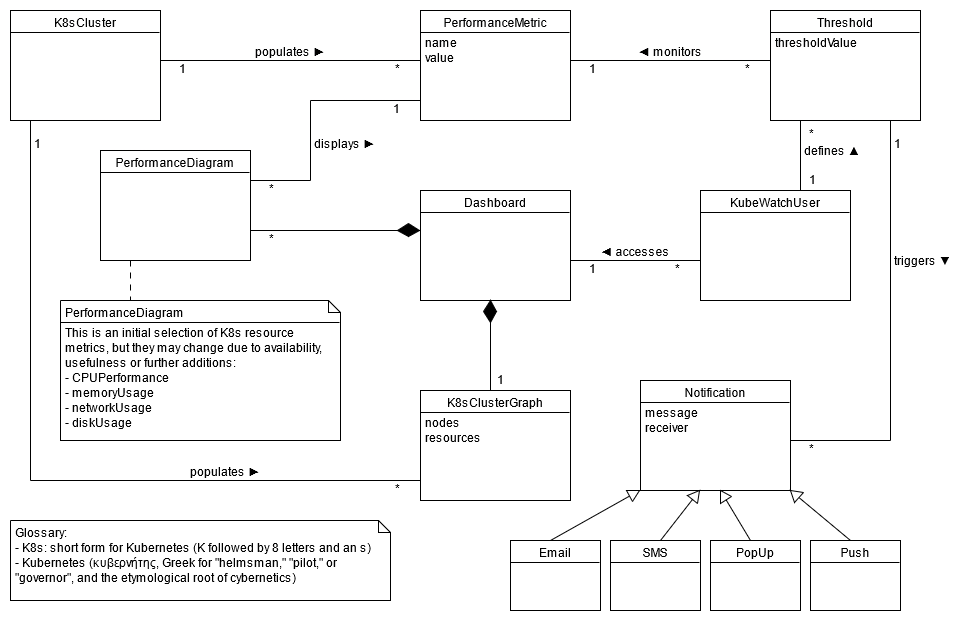
\includegraphics[width=\textwidth]{resources/domain_model.png}
\end{figure}